% phys.tex -- two colliding discs: from Newton's law to the impulse used by
% imp2d (see ../CONCEPTS.md).  Build:  pdflatex phys.tex  (twice for refs)
\documentclass[a4paper,11pt]{article}

\usepackage[margin=2.3cm]{geometry}
\usepackage{amsmath,amssymb,bm}
\usepackage{booktabs}
\usepackage{enumitem}
\usepackage{tikz}
\usetikzlibrary{arrows.meta,calc}

\setlist{itemsep=2pt,topsep=4pt}

\newcommand{\x}{\bm{x}}
\newcommand{\vV}{\bm{v}}
\newcommand{\VV}{\bm{V}}
\newcommand{\Jimp}{\bm{J}}
\newcommand{\hh}{\hat{n}}
\newcommand{\ttt}{\hat{t}}
\newcommand{\pp}{\bm{p}}          % linear momentum p = m v
\newcommand{\PP}{\bm{P}}          % total momentum, P = sum p over a set of bodies
\newcommand{\rr}{\bm{r}}          % lever arm: contact point relative to the centre
\newcommand{\dtc}{\Delta t_c}     % duration of the contact (NOT the substep \Delta t)
\newcommand{\dd}{\mathrm{d}}
\newcommand{\cn}{\text{(neg.\ if approaching)}}

\title{\bfseries Two colliding discs\\[4pt]
\large From $\bm{m\,\dot v=\sum F}$ to the impulse computed in
\texttt{sim.c}\\[10pt]
\normalsize\normalfont\itshape
Supporting derivation for \texttt{imp2d/CONCEPTS.md}.
The worked example uses the numbers of \texttt{selftest()} check~4.}
\author{}
\date{}

\begin{document}
\maketitle
\vspace{-2.6cm}

%--------------------------------------------------------------------------
\section{Statement of the goal}

Two rigid, smooth, coplanar discs $i$ and $j$ touch for a very short time.
We want the velocities right after the touch, starting from
\begin{equation}
  m_i\,\frac{\dd \vV_i}{\dd t}=\sum \bm{F},
  \qquad
  I_i\,\frac{\dd\omega_i}{\dd t}=\sum\tau_i=\sum\rr_i\times\bm F
  \label{eq:newton}
\end{equation}
and ending with the single line that \texttt{sim.c:365} computes,
\begin{equation}
  j_n=-\,(1+e)\,v_n\Big/\!\left(\frac{1}{m_i}+\frac{1}{m_j}\right) ,
  \qquad
  \Delta\vV_i=-\frac{j_n}{m_i}\,\hh,\quad
  \Delta\vV_j=+\frac{j_n}{m_j}\,\hh .
  \label{eq:goal}
\end{equation}
where
% The symbol list is set in from both margins --- a hanging block that is
% visibly narrower than the running prose around it.
\begin{description}[style=sameline, itemsep=3pt,
                    labelwidth=*, labelindent=1.8em, leftmargin=!,
                    rightmargin=2.4em]
  \item[$t$] time. $\dtc=t^{+}-t^{-}$ is the (vanishingly short) duration of the
    contact, $\Delta t=1/240$ s the substep of \texttt{sim\_step()};
    $\Delta t$ survives in the integration of gravity and \emph{not} in
    \eqref{eq:goal}.
  \item[$m_i$, $m_j$] masses of the two discs, constant during an impact
    (rigidity: a body neither gains nor loses mass). Spawned as
    $m=\rho r^{k}$ with $\rho=$ \texttt{--density} and $k=$
    \texttt{--mass-exp} $\in\{1,2,3\}$, so $k=2$ is the physical law for
    coplanar discs of constant areal density.
  \item[$\vV_i$, $\vV_j$] velocity of the \emph{centre} of each disc,
    $\vV=(v_x,v_y)$ in px/s --- a rigid disc has no other translational degree
    of freedom; $\Delta\vV_{i}$, $\Delta\vV_{j}$ are the velocity jumps that
    \eqref{eq:goal} produces.
  \item[$\pp=m\vV$, $\PP$] linear momentum of one disc, capital $\PP$ for
    the total of a set, $\PP=\sum\pp$. An \emph{impulse} is exactly a
    momentum transfer, $\Delta\pp=\Jimp$, which is why impulse and momentum
    share units here (mass$\cdot$px/s).
  \item[$\omega_i$, $\omega_j$] angular velocity (rad/s) about the axis through
    the centre, perpendicular to the plane. Positive $\omega$ turns a disc
    \emph{clockwise as seen on screen} ($y$ is down). The angle $\theta$ itself
    is integrated for the renderer only --- the solver reads $\omega$, never
    $\theta$.
  \item[$I_i$, $I_j$] moment of inertia about the body's \emph{own} centre; for
    a solid disc $I=\tfrac12 m r^{2}$, whence the identity $r^{2}/I=2/m$ used
    repeatedly below (and the reason $k_t=3k_n$ in \eqref{eq:kt3}).
  \item[$\sum\bm F$] total force on the body: the contact force plus everything
    non-impulsive (gravity, walls). Section~\ref{sec:jump} shows which part of
    this sum survives $\dtc\to0$.
  \item[$\tau$] torque --- a scalar in planar motion: $\tau=\rr\times\bm F$, with
    $\bm a\times\bm b=a_xb_y-a_yb_x$ the 2D \emph{scalar} cross product. The
    lever arm $\rr$ is the point where $\bm F$ acts, measured from the body's
    \emph{own centre}: at a disc surface $\rr_i=r_i\hh$, so $|\rr_i|$ happens to
    be the radius $r_i$ (bold $\rr$ the vector, plain $r_i$ the radius), and
    $\rr$ is \texttt{px, py} in \texttt{sim.c}. Equation \eqref{eq:newton} sums
    $\sum\tau$ over the forces on the body; that sum is what makes friction spin
    the discs.
  \item[$\hh$] contact unit normal, the direction of the line of centres,
    $\hh=(\x_j-\x_i)/d$ with $d=|\x_j-\x_i|$, pointing from $i$ to $j$
    \eqref{eq:geometry}. The impulse is along $\hh$; the geometry is the only
    place the discs' positions enter.
  \item[$v_n$] relative normal velocity $v_n=(\vV_j-\vV_i)\cdot\hh$, in px/s:
    negative $\Longleftrightarrow$ approaching \eqref{eq:vn}. It is the single
    scalar that the whole normal solve is driven by.
  \item[$e$] coefficient of restitution, $e\in[0,1]$ (\texttt{--rest}): $e=1$
    elastic, $e=0$ perfectly inelastic along $\hh$. A user constant, not a state
    variable --- the same value for walls and for pairs.
  \item[$j_n$] the \emph{scalar normal impulse}: the momentum (mass$\cdot$px/s,
    not newtons --- no force appears anywhere) that the contact delivers along
    $\hh$. One number serves both bodies: $+j_n\hh$ on $j$, $-j_n\hh$ on $i$
    (Newton's third law), which is why the system closes with a single unknown.
  \item[$1/m_i+\dfrac{1}{m_j}$] the \emph{normal effective mass} $k_n$ of the
    contact --- impulse required per unit of relative normal velocity
    \eqref{eq:kn}; its reciprocal $m_{\text{eff}}=1/k_n= m_im_j/(m_i+m_j)$ is
    the reduced mass. Inverse masses in the denominator are what split the
    velocity change as $|\Delta\vV_i|:|\Delta\vV_j|=m_j:m_i$.
\end{description}

\noindent
\textbf{Units and index conventions used throughout.} All quantities are in the
solver's own units --- pixels and seconds, never SI --- since the simulation
\emph{is} the physical model here; a subscript always names the disc the
quantity belongs to; a superscript $-$ or $+$ marks the state immediately
before or immediately after the impact; and $\Delta(\cdot)=(\cdot)^{+}-(\cdot)^{-}$
is the jump across the impact, not a small number.

Symbols introduced later, as they are needed: $\ttt=(-n_y,n_x)$ the contact
tangent, $v_{\text{slip}}$ the relative \emph{surface} velocity along $\ttt$,
$j_t$ and $k_t$ the tangential impulse and its effective mass, $\mu$ the Coulomb
coefficient (\texttt{--mu}), $\delta=r_i+r_j-d$ the penetration and $\beta$ the
strength of its positional correction.

Along the way: why the contact \emph{force} disappears, why momentum is
conserved exactly, when kinetic energy can and cannot grow, why the mass ratio
appears as an inverse-mass ratio, and how the same algebra with rotation gives
the friction/spin update.

\subsection{Conventions}
Positions are screen pixels, $x$ right and $y$ \emph{down}; the figures are
drawn in the usual mathematical orientation (a reflection does not change any
of the algebra). With the scalar cross product defined above,
$\hh\times\ttt=+1$, and an angular velocity about the axis perpendicular to the
plane acts as $\bm\omega\times\rr=\omega\,(-r_y,\,r_x)$.

%--------------------------------------------------------------------------
\section{Impulsive and non-impulsive forces}

Let the contact last $[t^-,\,t^+]$, of duration $\dtc=t^+-t^-$.
Equation \eqref{eq:newton} for body $i$ reads, with the contact force
$\bm F_{j\to i}$ from $j$ and everything else collected in $\bm F_i^{\text{ext}}$
(gravity, walls),
\begin{equation}
  m_i\bigl(\vV_i^+-\vV_i^-\bigr)
  =\underbrace{\int_{t^-}^{t^+}\bm F_{j\to i}(t)\,\dd t}_{\textstyle \Jimp_{j\to i}}
  \;+\;\int_{t^-}^{t^+}\bm F_i^{\text{ext}}(t)\,\dd t .
  \label{eq:integrated}
\end{equation}

Rigid-body impacts are idealisations: as $\dtc\to0$ the contact force grows
without bound while its \emph{integral} stays finite
($|\bm F_{j\to i}|\sim 1/\dtc$). Such a force is called \textbf{impulsive}, and
its integral is the \textbf{impulse}
\begin{equation}
  \Jimp:=\int_{t^-}^{t^+}\bm F\,\dd t
  \qquad[\text{units: mass}\cdot\text{px/s}].
  \label{eq:impulse}
\end{equation}
Gravity is bounded, $|\bm F^{\text{ext}}|\le m g$, so its integral is
$O(\dtc)\to 0$: it is \textbf{non-impulsive} and drops out of the impact
(Section~\ref{sec:jump} carries out both limits explicitly).
That is the precise sense in which ``a bounce does not feel gravity'', and it is
why \texttt{sim\_step()} is an \emph{operator split} (first-order Lie
splitting):
\[
  \vV \leftarrow \vV+\bm g\,\Delta t
  \qquad\text{then}\qquad
  \vV \leftarrow \vV+\Jimp/m \ \text{for each active contact}.
\]
From here on only impulsive quantities appear, and time no longer does:
\textbf{the solver changes velocities, never positions, and never uses forces.}

\subsection{How exactly does $m\,\dd\vV/\dd t$ become $m(\vV^+-\vV^-)$?}
\label{sec:jump}

Three operations; each is where a subtlety hides, so they are done one at a time.

\paragraph{Step 0 --- what $t^\pm$ and $\vV^\pm$ are.}
Let $t_c$ be the instant the discs first touch and let the contact release at
$t_c+\dtc$. The symbols $\vV^\pm$ are \emph{one-sided limits},
\[
  \vV^-=\lim_{\varepsilon\to0^+}\vV(t_c-\varepsilon),
  \qquad
  \vV^+=\lim_{\varepsilon\to0^+}\vV(t_c+\dtc+\varepsilon):
\]
the state the moment before the touch and the moment after the release. Between
them $\vV$ is not differentiable --- it is exactly the quantity that
\textbf{jumps}. One may therefore not differentiate \emph{through} the contact;
one integrates \emph{across} it and keeps only the endpoints. (In the solver the
two states are simply ``velocity entering the contact solve'' and ``velocity
after the impulse has been applied'', both inside one substep.)

\paragraph{Step 1 --- integrate over a window containing the whole contact.}
Choose $t^-<t_c$ and $t^+>t_c+\dtc$ and integrate \eqref{eq:newton} for body
$i$ term by term:
\begin{equation}
  \underbrace{\int_{t^-}^{t^+} m_i\,\frac{\dd\vV_i}{\dd t}\,\dd t}_{\text{(I)}}
  \;=\;
  \underbrace{\int_{t^-}^{t^+}\bm F_{j\to i}(t)\,\dd t}_{\text{(II)}}
  \;+\;
  \underbrace{\int_{t^-}^{t^+}\bm F_i^{\text{ext}}(t)\,\dd t}_{\text{(III)}} .
  \label{eq:window}
\end{equation}
Equality of functions implies equality of their integrals over any window, so
nothing has been assumed yet: all the physics is pushed into \emph{what
survives} when the window is squeezed down around the contact.

\paragraph{Step 2 --- (I) is an exact differential.}
A rigid body neither gains nor loses mass, so $m_i$ is a constant and comes out
of the integral. What is left is the fundamental theorem of calculus; written as
a substitution $\bm u=\vV_i(t)$, $\dd\bm u=(\dd\vV_i/\dd t)\,\dd t$, it is
\emph{path-independent}:
\begin{equation}
  \text{(I)}\;=\;m_i\int_{t^-}^{t^+}\frac{\dd\vV_i}{\dd t}\,\dd t
  \;=\;m_i\!\int_{\vV_i(t^-)}^{\vV_i(t^+)}\!\!\dd\bm u
  \;=\;m_i\bigl[\vV_i(t^+)-\vV_i(t^-)\bigr]
  \;=\;m_i\,\Delta\vV_i .
  \label{eq:ftc}
\end{equation}
Note what this buys: \textbf{the left side cannot see how the velocity got from
$\vV^-$ to $\vV^+$}. Force law, contact duration, deformation, even the order in
which the two discs deform --- all invisible on this side. That is precisely the
licence an impulse solver exploits to replace a whole event by one vector.

\paragraph{Step 3 --- what survives of (II) and (III).}
Classify the forces by their behaviour as the contact duration $\dtc\to0$:
\begin{center}
\scriptsize
\begin{tabular}{@{}llll@{}}
\toprule
force & size on the contact window & its integral & survives? \\
\midrule
$\bm F^{\text{ext}}$ (gravity, \dots) & $\le B$, independent of $\dtc$
  & $\le B\,\dtc\to0$ & no \\
$\bm F_{j\to i}$, contact, finite $\Delta\vV$ & $\sim C/\dtc$
  & $\to\Jimp=O(1)$ & \textbf{yes} \\
hypothetical $\sim C/\dtc^{\,p}$, $p>1$ & --- & $\to\infty$ & unphysical
  (infinite jump) \\
\bottomrule
\end{tabular}
\end{center}
Formally, with $|\bm F_i^{\text{ext}}|\le B$ on the window,
\[
  \biggl|\int_{t^-}^{t^+}\bm F_i^{\text{ext}}\,\dd t\biggr|
  \;\le\; B\,(t^+-t^-)\;\xrightarrow[\ \dtc\to0\ ]{\ }\;0 ,
\]
whereas the contact integral tends to the finite vector $\Jimp$
of \eqref{eq:impulse} --- that is what ``impulsive'' means. So \eqref{eq:window}
collapses to
\[
  \text{(I)}=\text{(II)}+\text{(III)}
  \quad\Longrightarrow\quad
  m_i\,\Delta\vV_i=\Delta\pp_i=-\Jimp+\bm 0 ,
\]
which is \eqref{eq:integrated} with its second integral gone: the momentum
$\pp_i=m_i\vV_i$ of body $i$ has changed by exactly the impulse it received.
The same computation for body $j$ gives $\Delta\pp_j=+\Jimp$, and Newton's
third law is what makes the two impulses one unknown.

\paragraph{Distribution wording (the same argument in one line).}
A rigid impact makes $\vV$ a step function,
$\vV_i(t)=\vV_i^{\text{reg}}(t)+H(t-t_c)\,\Delta\vV_i$ with $H$ the Heaviside
step, hence
$\dd\vV_i/\dd t=\dot\vV_i^{\text{reg}}+\delta(t-t_c)\,\Delta\vV_i$: the
acceleration carries a Dirac delta. The $\delta$-shaped contact force balances
$m\,\delta\,\Delta\vV$, and the bounded parts balance the bounded forces.
Integrating over a window that contains $t_c$ uses $\int\delta=1$ --- which is
Step 2 plus Step 3 compressed.

\paragraph{What the code does instead of taking a limit.}
\texttt{imp2d} never lets $\dtc\to0$; a substep is $\Delta t=1/240$ s and the
contact is assumed to complete \emph{within} it. Both halves of
\eqref{eq:window} are then handled, in the order of \texttt{sim\_step()}, but
\emph{differently}:
\begin{itemize}
\item \textbf{Non-impulsive forces are integrated by quadrature.} With
  $\bm F=m\bm g$ constant on a step, (III) $\approx m\bm g\,\Delta t$, so
  $m\,\Delta\vV=m\bm g\,\Delta t$, i.e.\ $\Delta\vV=\bm g\,\Delta t$ --- the line
  \texttt{b->vy += s->gravity * dt}. Numerically
  $1000\cdot\frac{1}{240}=4.2$ px/s per substep: the speed at which a resting
  ball re-arrives at its neighbour, hence the $10^{1}$ px/s scale of the pile
  jitter measured by \texttt{--stress}.
\item \textbf{Contact forces are never integrated.} There is no
  $\bm F\,\Delta t$ for a contact anywhere in the source: $\Jimp$ is obtained
  from the post-impact condition instead (Section~\ref{sec:restitution}), so the
  bounce does not depend on $\Delta t$ at all --- the same hit receives the same
  impulse at 60, 240 or 480 Hz. Only \eqref{eq:ftc} was used; no force, no
  duration.
\end{itemize}
Same law $\Delta\pp=\sum\Jimp$ in both cases; the difference is only \emph{how
the impulse is produced} --- rectangle rule for gravity, constraint solve for
contacts. That asymmetry is the whole reason a fixed-$\Delta t$ impulse solver
can be both stable and time-step-independent.
\subsection{The impulse--momentum relation}
With the limit of Section~\ref{sec:jump} taken, the non-impulsive term of
\eqref{eq:integrated} is gone; doing the same computation for body $j$:
\begin{equation}
  \boxed{\;
  \Delta\pp_i=m_i\,\Delta\vV_i=-\Jimp,\qquad
  \Delta\pp_j=m_j\,\Delta\vV_j=+\Jimp \;}
  \qquad\Longleftrightarrow\qquad
  \boxed{\;\Delta\pp=\textstyle\sum\Jimp\;}
  \label{eq:impulse-momentum}
\end{equation}
where $\pp=m\vV$ and $\Jimp$ is the impulse \emph{$i$ receives from $j$}, taken
with sign so that a compressive hit has $\Jimp$ along $+\hh$ on $j$. The second
box is the general statement --- sum over all contacts active in the substep,
plus the non-impulsive gravity term written as $m\,\bm g\,\Delta t$ --- of which
the first box is the two-body specialisation. Note what entered and what did
not:
\begin{itemize}
\item \emph{entered}: Newton's third law, $\Jimp_{i\leftarrow j}=-\Jimp_{j\leftarrow i}$,
  which is what makes $\Jimp$ a single unknown vector for the pair;
\item \emph{did not enter}: any detail of the contact force history. The rest of
  the derivation is supplied by one extra physical postulate (restitution) and
  the geometry of the contact.
\end{itemize}

%--------------------------------------------------------------------------
\section{Contact geometry}

At the (single) contact point $C$, with centre positions $\x_i,\x_j$ and
distance $d=|\x_j-\x_i|$,
\begin{equation}
  \hh=\frac{\x_j-\x_i}{d},\qquad
  \ttt=(-n_y,\,n_x),\qquad
  \delta=r_i+r_j-d ,
  \label{eq:geometry}
\end{equation}
$\hh$ points from $i$ to $j$, $\ttt$ is the contact tangent, and $\delta>0$ is
the \textbf{penetration} that the discrete time step necessarily produces
(Figure~\ref{fig:geom}). Any planar vector splits as
$\bm a=(\bm a\cdot\hh)\hh+(\bm a\cdot\ttt)\ttt$; we care about the
\textbf{relative normal velocity}
\begin{equation}
  v_n=(\vV_j-\vV_i)\cdot\hh ,
  \qquad
  v_n<0 \Longleftrightarrow \text{the discs are approaching}.
  \label{eq:vn}
\end{equation}

\begin{figure}[h]
\centering
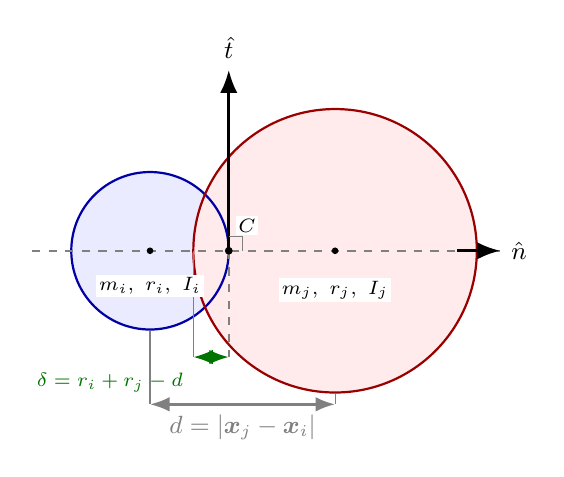
\begin{tikzpicture}[>=Latex, line width=0.9pt, font=\small]
  \def\Ri{1.0}                       % small disc, cm
  \def\Rj{1.8}                       % big disc, cm
  \def\pen{0.45}                     % penetration, cm
  \def\xB{\Ri+\Rj-\pen}              % x of j's centre; its left edge: \xB-\Rj
  \coordinate (A) at (0,0);
  \coordinate (B) at (\xB,0);
  \coordinate (C)  at (\Ri,0);        % right edge of i = contact point

  \fill[blue!8] (A) circle (\Ri);
  \fill[red!8]  (B) circle (\Rj);
  \draw[thick,blue!65!black] (A) circle (\Ri);
  \draw[thick,red!60!black]  (B) circle (\Rj);

  % the normal = line of centres, arrow drawn outside both bodies
  \draw[dashed,gray] (-1.5,0) -- (4.45,0);
  \draw[->,very thick] (3.9,0) -- (4.45,0) node[right,font=\small] {$\hh$};

  % the tangent at C
  \draw[->,very thick] (C) -- (1.0,2.3) node[above,font=\small] {$\ttt$};
  \draw[dashed,gray] (1.0,0) -- (1.0,-1.35);
  \draw[gray,thin] (1.18,0) -- (1.18,0.18) -- (1.0,0.18);
  \fill (C) circle (1.4pt);
  \node[fill=white,inner sep=1pt,font=\scriptsize,anchor=west]
       at (1.07,0.32) {$C$};

  % centre-to-centre distance d
  \draw[gray,thin] (0,-1.02) -- (0,-1.95);
  \draw[gray,thin] (\xB,-1.82) -- (\xB,-1.95);
  \draw[<->,gray] (0,-1.95) -- (\xB,-1.95)
        node[midway,below,font=\small] {$d=|\x_j-\x_i|$};

  % penetration delta: between the two boundary crossings along n
  \draw[gray,thin] ({\xB-\Rj},0) -- ({\xB-\Rj},-1.35);
  \draw[<->,green!45!black] ({\xB-\Rj},-1.35) -- (1.0,-1.35)
        node[anchor=north east,font=\scriptsize] at ({\xB-\Rj},-1.42)
        {$\delta=r_i+r_j-d$};

  \fill (A) circle (1.2pt);
  \node[fill=white,inner sep=1pt,font=\scriptsize] at (0,-0.45)
       {$m_i,\ r_i,\ I_i$};
  \fill (B) circle (1.2pt);
  \node[fill=white,inner sep=1pt,font=\scriptsize] at (\xB,-0.5)
       {$m_j,\ r_j,\ I_j$};
\end{tikzpicture}
\caption{Two discs, slightly interpenetrating (the state a discrete step
produces). The horizontal dashed line is the line of centres, whose direction is
$\hh$; the vertical arrow through $C$ is the contact tangent $\ttt$. The impact
algebra only ever uses $\hh$ and the scalar $v_n=(\vV_j-\vV_i)\cdot\hh$. A pair
of discs has exactly \emph{one} contact point, which is what keeps the solver
one scalar per pair.}
\label{fig:geom}
\end{figure}

%--------------------------------------------------------------------------
\section{Closing the system: Newton's restitution law}
\label{sec:restitution}

Equations \eqref{eq:impulse-momentum} leave the vector $\Jimp$ unknown: three
scalar unknowns in 2D ($\Jimp$ has two components, and one more if rotation is
involved). One postulate per contact direction closes it. Along the normal we
use \textbf{Newton's (Poisson's) impact law}: the approach speed along $\hh$ is
reversed and scaled by the coefficient of restitution $e\in[0,1]$,
\begin{equation}
  v_n^{+}=-\,e\,v_n^{-}.
  \label{eq:restitution}
\end{equation}
Write the impulse as $\Jimp=j\,\hh$ (a smooth contact with no friction has no
reason to push tangentially). From \eqref{eq:impulse-momentum},
\begin{align}
  \vV_i^{+}&=\vV_i^{-}-\frac{j}{m_i}\,\hh, &
  \vV_j^{+}&=\vV_j^{-}+\frac{j}{m_j}\,\hh , \notag\\[2pt]
  v_n^{+}&=(\vV_j^{+}-\vV_i^{+})\cdot\hh
        =v_n^{-}+j\underbrace{\left(\frac{1}{m_i}+\frac{1}{m_j}\right)}
        _{\textstyle :=\,k_n} . \label{eq:kn}
\end{align}
$k_n$ is the \textbf{normal effective mass} of the contact: the impulse needed
for one unit of relative normal velocity. Imposing \eqref{eq:restitution},
\[
  v_n^{-}+j\,k_n=-e\,v_n^{-}
  \quad\Longrightarrow\quad
  \boxed{\;j=-\,(1+e)\,\frac{v_n^{-}}{k_n}
        =-\,(1+e)\,m_{\text{eff}}\,v_n^{-}\;}
  \qquad
  m_{\text{eff}}:=\frac{1}{k_n}=\frac{m_i m_j}{m_i+m_j},
\]
which is \eqref{eq:goal}. Since $v_n^{-}<0$ at an approaching contact, $j>0$:
the impulse pushes the discs apart. It is \textbf{one-sided} --- the solver
applies it only when the pair overlaps \emph{and} $v_n^{-}<0$, and never pulls,
because a contact cannot carry tension.

\subsection{Variational meaning (why inverse masses appear)}
The same $j$ is the unique minimum-effort solution of
\begin{equation}
  \min_{\Delta\vV_i,\Delta\vV_j}\;
  \tfrac12 m_i|\Delta\vV_i|^2+\tfrac12 m_j|\Delta\vV_j|^2
  \quad\text{s.t.}\quad
  \bigl(\vV_j+\Delta\vV_j-\vV_i-\Delta\vV_i\bigr)\cdot\hh=-e\,v_n^{-},
  \label{eq:variational}
\end{equation}
i.e. among all velocity corrections that satisfy the impact law, take the one
that changes the kinetic energy as little as possible (measured in the kinetic
metric $\mathrm{diag}(m_i,m_j)$). Stationarity of the Lagrangian gives
$m_i\Delta\vV_i+\lambda\hh=0$ and $m_j\Delta\vV_j-\lambda\hh=0$, hence
$\Delta\vV_i=-(\lambda/m_i)\hh$, $\Delta\vV_j=(+\lambda/m_j)\hh$ --- equal and
opposite impulse, velocity change $\propto 1/m$ --- and the constraint yields
$\lambda=j$. This is why ``impulse solvers'' always look like
$\sum 1/m$ in the denominator.

%--------------------------------------------------------------------------
\section{What is conserved, what is not}

\subsection{Linear momentum: exactly, always}
Summing \eqref{eq:impulse-momentum} over the pair,
\begin{equation}
  \Delta\PP:=\Delta\bigl(\pp_i+\pp_j\bigr)=-\Jimp+\Jimp=\bm 0 ,
  \qquad\boxed{\;\Delta\PP=\bm 0\ \text{for any }e,\mu.}
  \label{eq:momentum}
\end{equation}
and for the whole system $\Delta\PP=\bigl(\sum_{\text{pairs}}\bm 0\bigr)
+\bigl(\text{wall impulses}\bigr)+\bigl(\sum m\,\bm g\,\Delta t\bigr)$: internal
contacts cannot move the centre of mass. This is a structural property, not a
tolerance --- it is what the selftest measures to $2\%$ (round-off only).
Equivalently, by K{\H o}nig's theorem the kinetic energy splits as
\begin{equation}
  KE=\underbrace{\tfrac12 M|\VV_{\text{cm}}|^2}_{\text{untouched by a pair}}
    +\underbrace{\tfrac12 m_{\text{eff}}\,v_n^{2}}_{\text{relative, normal}}
    +\underbrace{\tfrac12 m_{\text{eff}}\,v_{\tan,\text{rel}}^{2}
    +\sum \tfrac12 I\omega^2}_{\text{relative, tangential + spin}},
  \quad M=m_i+m_j,
  \label{eq:konig}
\end{equation}
so a pair impulse can only ever rearrange or remove the \emph{relative} part.

\subsection{Kinetic energy: never grows iff $e\le1$}
Expanding $KE^{+}-KE^{-}$ with
$|\vV+\Delta\vV|^2=|\vV|^2+2\vV\cdot\Delta\vV+|\Delta\vV|^2$:
\begin{align}
  \Delta KE
  &= m_i\vV_i\!\cdot\!\Delta\vV_i+\tfrac12m_i|\Delta\vV_i|^2
   + m_j\vV_j\!\cdot\!\Delta\vV_j+\tfrac12m_j|\Delta\vV_j|^2 \notag\\
  &= -j\,(\vV_i\!\cdot\!\hh)+\frac{j^2}{2m_i}
   + j\,(\vV_j\!\cdot\!\hh)+\frac{j^2}{2m_j}
   = j\,v_n^{-}+\tfrac12 j^2 k_n , \notag\\[3pt]
  \Longrightarrow\quad
  \boxed{\;\Delta KE=-\,\frac{1-e^2}{2\,k_n}\,\bigl(v_n^{-}\bigr)^2\;}
  \label{eq:dKE}
\end{align}
\[
  \text{equivalently}\qquad
  \Delta KE=-\,\tfrac12\bigl(1-e^2\bigr)m_{\text{eff}}\bigl(v_n^{-}\bigr)^2 ,
\]
Read it with \eqref{eq:konig}: $\tfrac12 m_{\text{eff}}(v_n^-)^2$ is precisely
the normal relative kinetic energy, and the collision removes the fraction
$1-e^2$ of it. Hence
\begin{itemize}
\item $e=1$: $\Delta KE=0$ \emph{identically} --- an elastic table with no
  gravity and no friction keeps $100\%$ of its energy, exactly as the
  \texttt{--selftest} gate asserts;
\item $e<1$: dissipation is proportional to $1-e^2$ and to the square of the
  approach speed;
\item $e>1$: energy would be \emph{created} --- which is why \texttt{--rest} is
  clamped to $[0,1]$ at parse time.
\end{itemize}

\subsection{Special cases worth memorising}
\begin{table}[h]
\centering\footnotesize
\begin{tabular}{@{}ll@{}}
\toprule
case & result \\
\midrule
$e=1$, $m_i=m_j$ & normal components \emph{exchanged}; a head-on hit swaps the
  two velocities \\
$e=1$, $m_i=m_j$, $j$ at rest & $\vV_i^{+}=(\vV_i^{-}\!\cdot\ttt)\ttt$,\
  $\vV_j^{+}=(\vV_i^{-}\!\cdot\hh)\hh$: they leave at $90^\circ$ (billiards) \\
$e=0$ & $v_n^{+}=0$: both share the normal part of the centre-of-mass velocity
  (a ``dead'' hit) \\
$m_j\to\infty$ & $m_{\text{eff}}\to m_i$,\ $j\to(1+e)m_i|v_n|$: the \textbf{wall}
  limit (\texttt{walls()}) \\
$m_j\gg m_i$ & $|\Delta\vV_i|:|\Delta\vV_j|=m_j:m_i$: the light disc takes all
  of the velocity change \\
$\mu=0$ & tangential components and both $\omega$ are untouched \\
\bottomrule
\end{tabular}
\caption{Consequences of \eqref{eq:goal} and \eqref{eq:dKE}.}
\end{table}

%--------------------------------------------------------------------------
\section{Rotation: the tangential impulse and Coulomb friction}

A smooth contact pushes along $\hh$ only. Real contacts also resist sliding, and
because that resistance acts \emph{at the surface}, it produces torque: this is
the whole reason the balls in \texttt{imp2d} spin.

\subsection{Contact kinematics}
The velocity of the material point of disc $i$ sitting at $\rr_i=r_i\hh$
(relative to its centre) is
\begin{equation}
  \bm u_i=\vV_i+\bm\omega_i\times\rr_i,
  \qquad
  (\bm\omega\times\rr)\cdot\ttt=\omega\,(\rr\times\ttt),
  \qquad
  \rr_i\times\ttt=+r_i,\quad \rr_j\times\ttt=-r_j ,
\end{equation}
since $\hh\times\ttt=+1$. The \textbf{slip velocity} at the contact is
\begin{equation}
  v_{\text{slip}}=(\bm u_j-\bm u_i)\cdot\ttt
   =(\vV_j-\vV_i)\cdot\ttt-\omega_j r_j-\omega_i r_i .
  \label{eq:slip}
\end{equation}

\subsection{Solve for the tangential impulse}
Apply the pair $\mp j_t\ttt$ (i.e.\ $-j_t\ttt$ to $i$, $+j_t\ttt$ to $j$, again a
third-law pair, so momentum stays exact). The impulse--momentum relation
\eqref{eq:impulse-momentum} and its angular twin $I\,\Delta\omega=\tau=\rr\times\Jimp$
give
\begin{equation}
  \Delta\vV_i=-\frac{j_t}{m_i}\ttt,\quad
  \Delta\vV_j=+\frac{j_t}{m_j}\ttt,\quad
  \Delta\omega_i=-\frac{j_t\,r_i}{I_i},\quad
  \Delta\omega_j=-\frac{j_t\,r_j}{I_j}.
  \label{eq:tangential-applied}
\end{equation}
Substituting into \eqref{eq:slip},
\begin{equation}
  v_{\text{slip}}^{+}=v_{\text{slip}}^{-}+j_t\,k_t,
  \qquad
  k_t=\frac{1}{m_i}+\frac{1}{m_j}+\frac{r_i^{2}}{I_i}+\frac{r_j^{2}}{I_j},
  \label{eq:kt}
\end{equation}
$k_t$ being the \textbf{tangential effective mass}: the extra $r^2/I$ terms are
the price of having to accelerate the \emph{surface}, not the centre. For solid
discs $I=\tfrac12mr^2$, so $r^2/I=2/m$ and
\begin{equation}
  \boxed{\;k_t=3\,k_n\;}\qquad\text{(solid discs)}
  \qquad\text{and, against a wall,}\qquad k_t=\frac{3}{m}.
  \label{eq:kt3}
\end{equation}

\subsection{Coulomb's law and sticking}
Dry friction limits the tangential impulse by the normal impulse just applied,
\begin{equation}
  |j_t|\le\mu\,j_n ,
  \label{eq:coulomb}
\end{equation}
and the two regimes fall out of \eqref{eq:kt}:
\begin{align}
  \text{\textbf{sticking:}}&\quad
    j_t=-\frac{v_{\text{slip}}^{-}}{k_t}\ \text{fits in \eqref{eq:coulomb}}
    \;\Rightarrow\; v_{\text{slip}}^{+}=0 \ \text{exactly};\\[2pt]
  \text{\textbf{sliding:}}&\quad
    j_t=-\mu\,j_n\,\operatorname{sgn}\!\bigl(v_{\text{slip}}^{-}\bigr)
    \ \Rightarrow\ \text{slip reduced, not removed.}
\end{align}
Writing $j_t=-\alpha\,v_{\text{slip}}^{-}/k_t$ with $\alpha\in[0,1]$ covers both,
and the energy change (now including the rotational terms; the cross terms
combine into \eqref{eq:slip} again) has the same shape as before:
\begin{equation}
  \Delta KE=j_t\,v_{\text{slip}}^{-}+\tfrac12 j_t^{2}k_t
          =-\Bigl(\alpha-\tfrac{\alpha^{2}}{2}\Bigr)
            \frac{\bigl(v_{\text{slip}}^{-}\bigr)^{2}}{k_t}\ \le\ 0 .
  \label{eq:friction-energy}
\end{equation}
So \textbf{friction can only remove energy} --- including spin energy --- and
the selftest's spin gate is a plain non-increase test on
$KE=\sum\bigl(\tfrac12 m|\vV|^2+\tfrac12 I\omega^2\bigr)$.

Two practical corollaries for tuning \texttt{--mu}:
\begin{equation}
  |\Delta\omega_i|=\frac{|j_t|\,r_i}{I_i}\le
  \frac{2\mu(1+e)\,m_{\text{eff}}\,|v_n|}{m_i\,r_i}
  \qquad\xrightarrow{\ \text{wall}\qquad}\qquad
  |\Delta\omega|\le\frac{2\mu(1+e)\,|v_n|}{r},
  \label{eq:dw}
\end{equation}
\begin{equation}
  \text{a contact \emph{sticks}}\iff
  \frac{|v_{\text{slip}}|}{k_t}\le\mu\,j_n
  \quad\Longleftrightarrow\quad
  |v_{\text{slip}}|\le 3\mu(1+e)\,|v_n|
  \label{eq:stick}
\end{equation}
(in \eqref{eq:stick} the $k_t=3k_n$ of \eqref{eq:kt3} was used, so the criterion
is the same for a disc--disc and a disc--wall contact).

With the defaults $\mu=0.2$, $e=0.9$, side slip below $\approx1.14$ times the
approach speed vanishes in a single bounce; above it the contact slides and
\eqref{eq:dw} saturates. Once $v_{\text{slip}}=0$ the disc \emph{rolls}
($\vV\cdot\ttt=\omega r$ in the wall case) and, there being no rolling
resistance here, it rolls forever.

%--------------------------------------------------------------------------
\section{Worked example (the selftest scene)}

Take the head-on case of \texttt{selftest()} check~4: same line, opposite
directions, elastic, no friction.
\[
  \rho=0.001,\quad r_i=10,\ r_j=30
  \;\Rightarrow\; m_i=0.1,\ m_j=0.9,
  \qquad v_i^{-}=+300,\ v_j^{-}=-100\ \text{px/s},\quad e=1 .
\]
Then $\hh=+\hat x$, $v_n^{-}=(-100)-(+300)=-400$ px/s,
$k_n=1/0.1+1/0.9=11.1111$, $m_{\text{eff}}=0.09$, so
\[
  j=-(1+1)\cdot0.09\cdot(-400)=\mathbf{72}
  \quad\Rightarrow\quad
  \Delta v_i=-\frac{72}{0.1}=-720,\qquad
  \Delta v_j=+\frac{72}{0.9}=+80,
\]
\[
  v_i^{+}=-420\ \text{px/s},\qquad v_j^{+}=-20\ \text{px/s}.
\]
Checks: $P^{-}=0.1\cdot300+0.9\cdot(-100)=-60=P^{+}=0.1\cdot(-420)+0.9\cdot(-20)$
(momentum exact); $v_n^{+}=-20-(-420)=+400=-v_n^{-}$ (restitution exact);
$KE^{-}=\tfrac12(0.1)(300^2)+\tfrac12(0.9)(100^2)=4500+4500=9000$ and
$KE^{+}=\tfrac12(0.1)(420^2)+\tfrac12(0.9)(20^2)=8820+180=9000$
($e=1$: nothing lost, \eqref{eq:dKE}); the heavy ball lost $80$ px/s of speed
while the light one reversed $720$ px/s --- the $m_j/m_i=9$ asymmetry of
\eqref{eq:impulse-momentum}. Figure~\ref{fig:beforeafter} shows the sequence.

\begin{figure}[h]
\centering
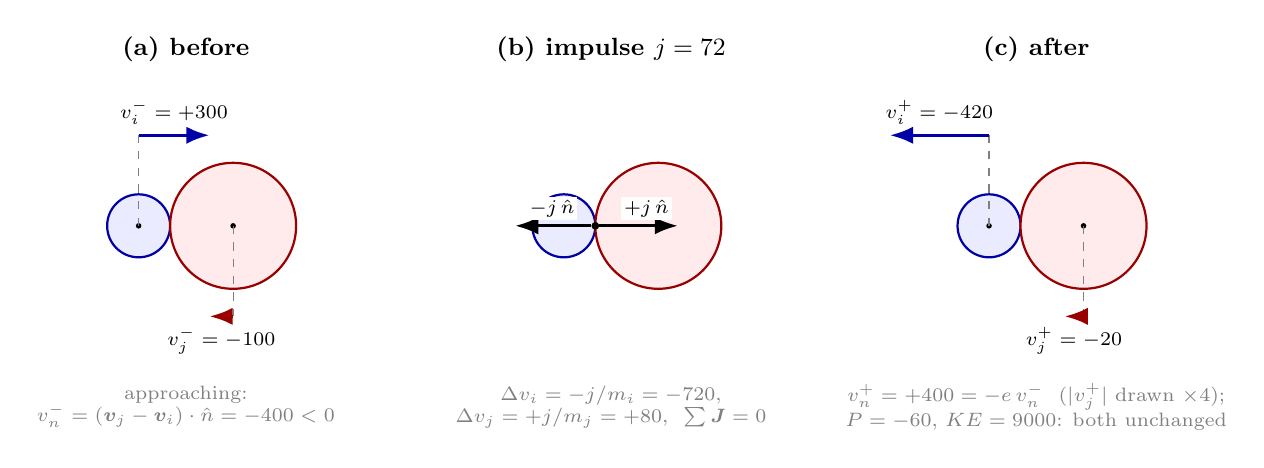
\begin{tikzpicture}[>=Latex, line width=0.9pt, font=\scriptsize]
  % Three panels. In each: light disc i (blue, r=0.4cm) touching heavy disc j
  % (red, r=0.8cm); line of centres is horizontal, \hh points right.
  % Velocity arrows are proportional to speed (0.003 cm per px/s) except
  % |v_j^+|, drawn x4 so that it is visible at all.
  \def\Ri{0.40}
  \def\Rj{0.80}
  \def\xj{\Ri+\Rj}
  \def\up{1.15}
  \def\dn{-1.15}

  % ---------------------------- (a) before --------------------------------
  \begin{scope}[xshift=0cm]
    \node[anchor=south,font=\small\bfseries] at (0.6,1.95) {(a) before};
    \fill[blue!8] (0,0) circle (\Ri);
    \draw[thick,blue!65!black] (0,0) circle (\Ri);
    \fill[red!8]  (\xj,0) circle (\Rj);
    \draw[thick,red!60!black]  (\xj,0) circle (\Rj);
    \fill (0,0) circle (1pt); \fill (\xj,0) circle (1pt);
    \draw[dashed,gray,thin] (0,0) -- (0,\up);
    \draw[->,very thick,blue!65!black] (0,\up) -- (0.90,\up)
        node[midway,above,black] {$v_i^{-}=+300$};
    \draw[dashed,gray,thin] (\xj,0) -- (\xj,\dn);
    \draw[->,very thick,red!60!black] (\xj,\dn) -- (\xj-0.30,\dn)
        node[midway,below,black] {$v_j^{-}=-100$};
    \node[align=center,text=gray] at (0.6,-2.30)
        {approaching:\\ $v_n^{-}=(\vV_j-\vV_i)\cdot\hh=-400<0$};
  \end{scope}

  % --------------------- (b) the impulse pair -----------------------------
  \begin{scope}[xshift=5.4cm]
    \node[anchor=south,font=\small\bfseries] at (0.6,1.95) {(b) impulse $j=72$};
    \fill[blue!8] (0,0) circle (\Ri);
    \draw[thick,blue!65!black] (0,0) circle (\Ri);
    \fill[red!8]  (\xj,0) circle (\Rj);
    \draw[thick,red!60!black]  (\xj,0) circle (\Rj);
    \fill (\Ri,0) circle (1.4pt);
    \draw[->,very thick] (\Ri-0.05,0) -- (-0.62,0)
        node[fill=white,inner sep=1pt] at (-0.15,0.22) {$-j\,\hh$};
    \draw[->,very thick] (\Ri+0.05,0) -- (\xj+0.25,0)
        node[fill=white,inner sep=1pt] at (1.05,0.22) {$+j\,\hh$};
    \node[align=center,text=gray] at (0.6,-2.30)
        {$\Delta v_i=-j/m_i=-720$,\\
         $\Delta v_j=+j/m_j=+80$, \ $\sum\Jimp=0$};
  \end{scope}

  % ---------------------------- (c) after ---------------------------------
  \begin{scope}[xshift=10.8cm]
    \node[anchor=south,font=\small\bfseries] at (0.6,1.95) {(c) after};
    \fill[blue!8] (0,0) circle (\Ri);
    \draw[thick,blue!65!black] (0,0) circle (\Ri);
    \fill[red!8]  (\xj,0) circle (\Rj);
    \draw[thick,red!60!black]  (\xj,0) circle (\Rj);
    \fill (0,0) circle (1pt); \fill (\xj,0) circle (1pt);
    \draw[dashed,gray,thin] (0,0) -- (0,\up);
    \draw[->,very thick,blue!65!black] (0,\up) -- (-1.26,\up)
        node[midway,above,black] {$v_i^{+}=-420$};
    \draw[dashed,gray,thin] (\xj,0) -- (\xj,\dn);
    \draw[->,very thick,red!60!black] (\xj,\dn) -- (\xj-0.24,\dn)
        node[midway,below,black] {$v_j^{+}=-20$};
    \node[align=center,text=gray] at (0.6,-2.30)
        {$v_n^{+}=+400=-e\,v_n^{-}$ \ ($|v_j^{+}|$ drawn $\times4$);\\
         $P=-60$, $KE=9000$: both unchanged};
  \end{scope}
\end{tikzpicture}
\caption{Head-on elastic hit of a light disc ($m_i=0.1$) on a heavy one
($m_j=0.9$). One impulse $j$, applied with opposite signs, does it all: the
light disc reverses hard, the heavy one barely notices, momentum and kinetic
energy are both exactly preserved because $e=1$.}
\label{fig:beforeafter}
\end{figure}

%--------------------------------------------------------------------------
\section{What the code adds on top of the algebra}

The closed-form pair impulse above is applied $O(\text{pairs})$ times per
substep, in a relaxation sweep, with three additions:

\begin{enumerate}[label=(\arabic*)]
\item \textbf{Order.} Contacts are resolved one at a time against the already
  updated state (Gauss--Seidel), repeated \texttt{ITER}$=2$ times. One sweep of
  \eqref{eq:goal} per pair is \emph{not} the solution of the simultaneous
  problem --- it is one relaxation pass; several would converge to an LCP
  solution.
\item \textbf{Positional projection.} Because \eqref{eq:impulse-momentum} never
  moves positions, the overlap $\delta$ from Figure~\ref{fig:geom} persists; it
  is removed geometrically, split by inverse mass exactly as the impulse is:
  \[
    \Delta\x_i=-\frac{\beta\,(\delta-\delta_0)}{k_n}\,\frac{1}{m_i}\,\hh,
    \qquad
    \Delta\x_j=+\frac{\beta\,(\delta-\delta_0)}{k_n}\,\frac{1}{m_j}\,\hh,
    \qquad \beta=0.8,\ \delta_0=0.01\ \text{px},
  \]
  which leaves $\sum m\,\Delta\x=0$: centre of mass, momentum and rotation
  untouched, no kinetic energy added (potential energy in a gravity field,
  however, can change --- the one energy loophole in the scheme).
\item \textbf{Friction is conditional.} \eqref{eq:tangential-applied} is applied
  only where a compressive $j_n$ was just produced, i.e. friction is caused by
  the normal impulse and bounded by it through \eqref{eq:coulomb}.
\end{enumerate}

\clearpage
\subsection{Equation $\to$ source}
\begin{center}
\scriptsize
\begin{tabular}{@{}lll@{}}
\toprule
equation & source & note \\
\midrule
guard $d^2>0$, $\hh$            & \texttt{sim.c:355--358} & \eqref{eq:geometry} \\
$v_n$, $k_n$                   & \texttt{sim.c:359--360} & \eqref{eq:vn}, \eqref{eq:kn} \\
one-sidedness $v_n<0$          & \texttt{sim.c:363}      & unilateral contact \\
$j=-(1+e)v_n/k_n$              & \texttt{sim.c:365}      & \eqref{eq:goal} \\
$\Delta\vV_{i,j}=\mp(j/m)\hh$  & \texttt{sim.c:366--369} & \eqref{eq:impulse-momentum} \\
$\ttt$, $\bm u_{i,j}$, $v_{\text{slip}}$, $k_t$
                               & \texttt{sim.c:268--276} & \eqref{eq:slip}, \eqref{eq:kt} \\
sticking $j_t=-v_{\text{slip}}/k_t$ & \texttt{sim.c:277} & \eqref{eq:coulomb} \\
clamp to $\pm\mu j_n$          & \texttt{sim.c:278--280} & \eqref{eq:coulomb} \\
$\Delta\vV$, $\Delta\omega=-j_t r/I$ & \texttt{sim.c:282--287} & \eqref{eq:tangential-applied} \\
friction only if $j_n\neq0$    & \texttt{sim.c:374}      & item (3) above \\
wall: $j_n=(1+e)m\|v_n\|$      & \texttt{sim.c:299,307,316,324} & $m_j\to\infty$ limit \\
$\delta$, positional projection& \texttt{sim.c:378--384} & item (2) above \\
$KE$, $\PP$                  & \texttt{sim.c:436,445}  & \eqref{eq:konig} \\
\bottomrule
\end{tabular}

\vspace{4pt}
{\small\itshape Where each derived formula lives.}
\end{center}

%--------------------------------------------------------------------------
\section*{Summary}
\addcontentsline{toc}{section}{Summary}
\vspace{-0.8em}
{\small
\begin{align*}
  m\dot{\vV}=\textstyle\sum\bm F
  &\ \xrightarrow[\ \dtc\to0\ ]{\ \int \dd t\ }\
   \Delta\pp=\textstyle\sum\Jimp,\quad\pp=m\vV
   \quad\text{(only impulsive forces survive)}\\
  \Jimp=j\hh,\quad v_n^{+}=-e\,v_n^{-}
  &\ \Longrightarrow\
   j=-\,(1+e)\,\frac{v_n^{-}}{1/m_i+1/m_j}
   \quad\text{(and }m\,\Delta\vV_i=-\Jimp=-m\,\Delta\vV_j\text{)}\\
  &\ \Longrightarrow\ \Delta\PP=0,\qquad
   \Delta KE=-\tfrac12(1-e^2)m_{\text{eff}}(v_n^{-})^2\le0 \iff e\le1,\\
  \Jimp=j_t\ttt\ \text{at the surface}
  &\ \Longrightarrow\ k_t=3k_n,\
   j_t=\operatorname{clamp}\!\bigl(-v_{\text{slip}}/k_t,\ \pm\mu j_n\bigr),\
   \Delta\omega=\tau/I=-j_t r/I,
\end{align*}
i.e.\ a mass-weighted, one-sided, momentum-exact velocity update --- which is
exactly what \texttt{sim.c} spends its inner loop doing.
}

\end{document}
